\documentclass[letterpaper, 11pt]{article}
\usepackage[letterpaper, margin=1.4in]{geometry}
\usepackage{amsmath, amssymb}
\usepackage{graphicx}
\usepackage{verbatimbox}
\usepackage{listings}
\lstset{
 basicstyle=\ttfamily,
 columns=fullflexible,
 frame=single,
 breaklines=true,
}
\usepackage{caption}
\usepackage{subcaption}

\title{ChatApp Design API Specification}
\author{Team Houston\\ Jonathan Wang, Manu Maheshwari, Yanjun Yang,\\ Tianqi Ma, Youyi Wei, Jiang Lin, Chengyin Liu}
\date{}

\setlength\parindent{0pt}

\begin{document}
\maketitle

We used the command, composite, and singleton design patterns for this Chat App. We have two controllers, the ChatAppController and the WebSocketController to handle the requests and communications. We also have two top-level classes, the ChatRoom and the User. The ChatAppController is an observable, observed by ChatRooms, and the ChatRoom is also an observable, observed by Users. All the objects use commands to act in the chat app. \\

In this document, we will discuss the use cases for the chat app. We will then break down the interfaces and classes in the model. 

\section{Use Cases}
\begin{itemize}
  \item Enter ChatApp
  \begin{itemize}
    \item Map session to new or existing user by username
  \end{itemize}
  \item Create ChatRoom
  \begin{itemize}
    \item Send request message with chat room restrictions
    \item Create chat room with user as owner
    \item Add chat room as observer of ChatAppController for users to determine relevant rooms
  \end{itemize}
  \item Join ChatRoom
  \begin{itemize}
    \item User can only see chat rooms that it can join
    \item Add user as observer of each room it joins so chat room know who is in room
  \end{itemize}
  \item Leave ChatRoom
  \begin{itemize}
    \item Exit one or all chat rooms
    \item Send message about why user left
    \item Update owner if owner leaves
  \end{itemize}
  \item Send message
  \begin{itemize}
    \item Regular users send message to one user in chat room
    \item Owner can send message to all users in chat room
    \item Notify message has been received
    \item Remove user if message contains 'hate'
    \item Display messages appropriately for appropriate users
  \end{itemize}
  \item Check ChatRooms User is in/can join, Users in ChatRoom
\end{itemize}

\section{View}
We have several sections in our ChatApp - a login, a chat room list, the chat room, and a create chat room form. Each interaction in the view makes a request to the model by having the websocket send a request message via the WebSocketController.

\section{Controller}
We have two controllers: ChatAppController and WebSocketController. 
\begin{itemize}
\item ChatAppController is an observable observed by chat rooms. It is also a singleton, so that the notifyObservers method can be accessed from WebSocketController. WebSocketController will call the ChatAppController instance to interact with the model.
\begin{itemize}
  \item sessionUsernameHashmap: a ConcurrentHashMap maps the session to the username.
  \item usernameUserHashmap: a ConcurrentHashMap maps the username to the user object.
  \item chatAppController: a singleton instance of itself.
  \item ChatAppController(): constructor.
  \item getInstance(): get singleton instance of ChatAppController.
  \item main(String[] args): ChatApp entry point.
  \item logIn(Session user, String request): creates a new user if user is not created or retrieves an existing user. Updates hashmaps accordingly.
  \item getEligibleChatRooms(Session user, String request): get all chatrooms user is in or can join. Send the lists as JSON to session.
  \item createChatRoom(Session user, String request): create a chat room. Send updated lists as JSON to session.
  \item joinChatRoom(Session user, String request): join a chat room. Send updated lists as JSON to session.
  \item getChatRoom(Session user, String request): get users in chat room and chat history. Send as JSON to  session.
  \item leaveChatRoom(Session user, String request): exit one or all chat rooms. Send updated lists as JSON to session.
  \item sendMessage(String request): send a message command to all the chat room observers.
  \item getHerokuAssignedPort(): get the heroku assigned port number.
\end{itemize}

\item WebSocketController creates a web socket for the server; it also manages all of the end points by parsing messages from the view. It then calls the appropriate methods in ChatAppController to interact with the model. We have seven end points:
\begin{itemize}
  \item ``log$\_$in": create or retrieve user in hash map.
  \item ``get$\_$eligible$\_$chat$\_$rooms": get list of chat rooms that user is in or can join.
  \item ``join$\_$chat$\_$room": join an existing chat room.
  \item ``get$\_$chat$\_$room": get users in chat room and message history when entering chat room.
  \item ``exit$\_$chat$\_$room": exit one or all chat rooms.
  \item ``create$\_$chat$\_$room": create chat room.
  \item ``send$\_$message": send message to user in chat room.
\end{itemize}
\end{itemize}

We have an important design decision here - all requests from the view go to the WebSocketController via the websocket send interface. The WebSocketController calls the appropriate methods in ChatAppController, which handles backend actions and sends a response back to the view as a message, allowing us to use Session as the single identifier from the view. 

\section{Model}
\subsection{Command}
We have one interface for the commands: ISndMsgCmd. This command will be executed by the Users and ChatRooms. It has one function: execute(Object context), which has the receiver (context) execute the command. All interactions between observables and their observers will be handled by the command design pattern.

\subsection{Objects}
We have two concrete objects: ChatRoom and User. ChatRoom is an observable and an observer that observes the ChatAppController. User is an observer that observes each ChatRoom it is in. CompositeUser and CompositeChatRoom extend each class to handle sending message to all users or leaving all chat rooms.

\section{Design}
We include two diagrams to show how the view and model communicate using the WebSocketController and ChatAppController. This flow is the primary design decision for the API. \\

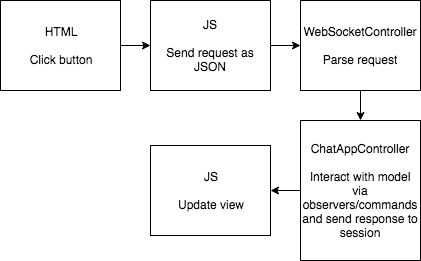
\includegraphics[width=\textwidth]{request_handling} \\
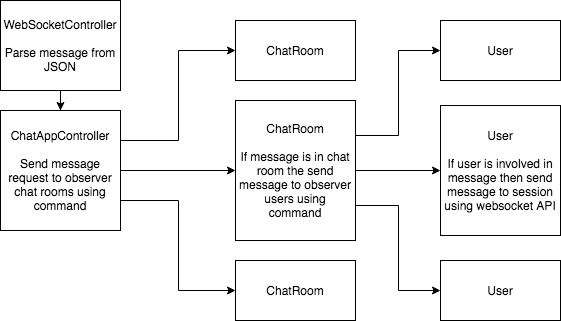
\includegraphics[width=\textwidth]{message_sending}

\end{document}